\section{HSL}

\subsection{C}
El código de C, al igual que el resto, es bastante sencillo. Lo que hace es loopear sobre todos los píxeles, hacer una conversión de RGB a HSL, hacer las sumas correspondientes, y luego volver a convertir a RGB.

Lo malo de la implementación es que el código sin optimizar de C hace más operaciones de las necesarias, ya que no usa todo el poder de las operaciones en SSE, que nosotros intentamos utilizar al máximo.

\subsection{ASM1}

En la versión primera versión del código de assembler la operatoria es bastante distinta a la de C.
Al principio calculamos en xmm4 el vector de números que debemos sumarle a cada pixel hsl, con los parámetros que nos pasaron. De esta manera, 

\xmm{4}
\regfloats{l}{s}{h}{0}

Donde h,s,l son los que nos pasaron como parámetro y el 0 es lo que le tenemos que sumar a la transparencia (nada). Este registro tenemos que guardarlo en la pila, dado que cuando llamamos a rgbTOhsl, nos puede pisar los registros xmm pues la convención C no especifica nada sobre que no se puedan pisar (de hecho en algunos casos lo pisa, fue un bug que tardamos en encontrar).

También tenemos que malloc'ear un float para llamar a las funciones rgbTOhsl y hslTOrgb. Podríamos usar la pila, pero nos resultó mas fácil usar este método.

Luego comenzamos a loopear. 

Luego de convertir el pixel en cuestión de rgb a hsl, vamos a tener su valor en \xmm{3}.

\xmm{3}
\regfloats{LL}{SS}{HH}{AA}

Luego sumamos este registro con el registro que contiene los parámetros, como indica el filtro, de manera que queda

\xmm{3}
\regfloats{l+LL}{s+SS}{h+HH}{AA}

Va a ser útil para mas adelante tener un ejemplo, así que supongamos que \xmm{3} vale

\xmm{3}
\regfloats{0.5}{-0.322}{380}{255}


Ahora comienza la operatoria de saturación, entonces vamos a armar los siguientes registros

\xmm{5}
\regfloats{1-(l+LL)}{1-(s+SS)}{-360}{0}

\xmm{6}
\regfloats{-(l+LL)}{-(s+SS)}{360}{0}

Siguiendo el ejemplo anterior, los registros quedarían

\xmm{5}
\regfloats{0.5}{1.322}{-360}{0}

\xmm{6}
\regfloats{-0.5}{0.322}{360}{0}



Entonces procedemos a formar estos registros, usando la menor cantidad de instrucciones posibles, como siempre.

Luego nos armamos 2 registros más, que vamos a usar para las comparaciones

\xmm{12}
\regfloats{1}{1}{360}{256}

\xmm{13}
\regfloats{0}{0}{0}{0}


Luego comparamos estos registros con nuestro registro \xmm{3} (nótese que como SSE carece de comparaciones de mayor o igual, hay que dar vuelta los registros y hacer una comparación de menor o igual).

Por lo tanto, con el ejemplo anterior, \xmm{12} y \xmm{13} quedan así:

\xmm{12}
\regfloats{0h}{0h}{ffffffffh}{0h}

\xmm{13}
\regfloats{0h}{ffffffffh}{0h}{0h}


Luego les hacemos un and entre los registros \xmm{12} y \xmm{5} y entre \xmm{13} y \xmm{6}, dword a dword, de manera seleccionar lo que vamos a querer sumar. En el ejemplo esto queda


\xmm{5}
\regfloats{0}{0}{-360}{0}

\xmm{6}
\regfloats{0}{0.322}{0}{0}

Recordemos el valor de \xmm{3}

\xmm{3}
\regfloats{0.5}{-0.322}{380}{255}


Ahora les sumamos estos registros a \xmm{3}, para terminar de llevar a cabo nuestro plan

\xmm{3}
\regfloats{0.5}{0}{320}{255}

Y listo, todo terminó como queríamos.

Ahora solo falta volver a convertir este numero a RGB y escribirlo a la memoria, de lo que se va a ocupar la función hslTOrgb.

\subsection{ASM2}

En la segunda implementación utilizamos fuertemente la primera.

Lo que hicimos en ambas rutinas de conversión es bastante directo, siguiendo los algoritmos proveídos por la cátedra. El mayor problema que tuvimos en ambas rutinas fue que tenemos que cargar constantemente constantes que vamos a usar durante los procesos. Esto hace que la ejecución de las rutinas de conversión sea mucho mas lenta de lo que podría ser si tuviéramos más registros para guardar las constantes que usamos todo el tiempo.

Este es definitivamente el factor más limitante de nuestra implementación y esperamos que impacte fuertemente en el rendimiento.


\pagebreak
\subsection{Experimentación}

Al igual que en los anteriores filtros, esperábamos que el rendimiento de nuestra implementación en assembler sea más rápida que la de C. Sin embargo los resultados nos dijeron lo contrario.


\begin{figure}[!hbt] 
	\centering
  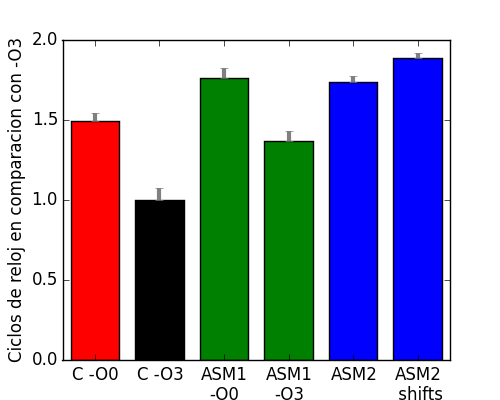
\includegraphics[width=10cm]{images/hsl.png}
  \caption{Comparación de la cantidad de ciclos de reloj utilizada por diferentes variantes de hsl. Para tener una medida absoluta: la cantidad de ciclos de reloj promedio de C -O3 es 31,620,627. Tamaño de la muestra: 200 imágenes de $16 \times 10^4$ píxeles. Se indica el mínimo con la barra y el promedio con una linea gris.}
\end{figure}

Los resultados fueron devastadores, dado que no los esperábamos. Al igual que el resto de los filtros, el comportamiento de los algoritmos es lineal sobre la cantidad de píxeles, pero la pendiente de nuestras implementaciones de assembler es mayor que las de C.

Por esta razón nos propusimos a hacer un amplio análisis de la situación, para poder descubrir la razón del bajo rendimiento.

La principal limitación de nuestra implementación de assembler son, claramente, los accesos a memoria. En cada rutina (de ambas implementaciones) debemos cargar muchas constantes que usaremos a lo largo de las distintas cuentas que debemos hacer.
Esto es muy caro para nosotros, dado que los accesos a memoria son de lo mas limitante en lo que concierne a la performance. 
A esto atribuimos principalmente nuestro pobre desempeño frente a la implementación de C. Veremos más adelante otras circunstancias que apoyan esta teoría.

Habiendo dicho esto, también es cierto que una vez que pedimos un dato de memoria, este debería guardarse en la cache, siendo su acceso mucho más rápido. Pero la cache sigue siendo aún mas lenta que los registros del procesador, por lo que acceder a memoria (por mas que sea cache) sigue siendo un factor limitante.
\\

Por otro lado, nuestros algoritmos no dependen fuertemente en saltos condicionales, usan los necesarios, por lo tanto no creemos que este sea un factor limitante del rendimiento.
\\

La siguiente limitación de nuestra implementación es la operatoria de las conversiones de RGB a HSL y viceversa. Esto se debe a que las operaciones que se deben hacer son largas y costosas, por mas que esten lo mejor optimizadas posibles.

A esto se le suma la dificultad de operar de a muchos píxeles juntos, dado que solo se puede en pequeñas partes.
Por ejemplo, en hslTOrgb se podría calcular de forma paralela c, x, m para 4 pixeles así como la operatoria de los shuffles.
Sin embargo, la complejidad del código crece enormemente, sumado a que la operación de rgbTOhsl y la de Suma no son así de simples de paralelizar.
Por estas razones, optamos por no probar esta variante del código, pero es una opción a tener en cuenta.
\\

Comentando partes de códigos, pudimos obtener una partición tentativa de cuanto tarda cada operación de la segunda implementación de hsl, algo que nos parece vital a la hora de analizar la performance. Los resultados fueron los siguientes:


\begin{figure}[H] 
	\centering
  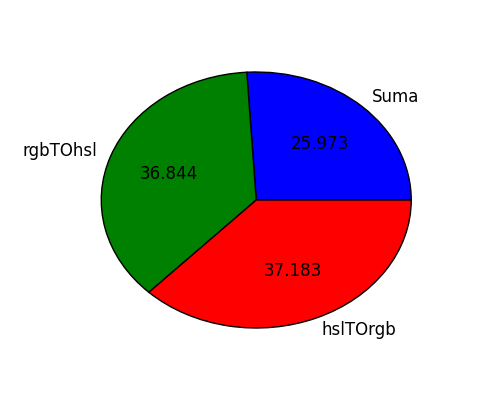
\includegraphics[scale=0.7]{images/hsl-div.png}
  \caption{Análisis comparativo del porcentaje de tiempo dedicado a cada instancia. Tamaño de la muestra: 100 imágenes de $16\times 10^4$ píxeles}
\end{figure}

Este gráfico debe interpretarse de la siguiente manera: el tiempo que se dedica en cada loop a hacer cada una de esas operaciones, es aproximadamente el indicado en el porcentaje.

A priori parecería que el proceso de Suma es más lento de lo que debería ser, lo cual es posible, dado que se cargan muchas veces las mismas cosas de memoria. Esto es inevitable en la primera implementación de hsl (dado que las llamadas a las funciones de C nos rompen todos los registros y no podemos guardar nada), mientras que podría ser evitable en la segunda implementación.

Sin embargo, viendo el código de nuestra implementación no parece que se pudiera mejorar demasiado (sin cambiar los algoritmos drásticamente), dado que los principales cambios que podrían realizarse son pasar de shifts a shuffles o extracts/inserts. Pero estas optimizaciones, como vimos anteriormente, no dan un speedup muy grande.
\\

Lo último que queda inspeccionar para encontrar una razón por la cual el código de C le gana al nuestro, es mirando el output de assembler de GCC. Para ello, corremos el comando \texttt{gcc -O3 -S -nasm=intel -fverbose-asm C\_hsl.c}.

Lo primero que se nota en el código de assembler outputeado por GCC es el uso de saltos condicionales. Como el código de este algoritmo depende fuertemente en condifionales (ifs), el hecho de poder utilizar saltos inteligentemente como lo puede hacer un compilador (en vez de máscaras como usamos nosotros) puede dar ventajas.

Otra posible explicación es que el código generado por GCC carga menos cosas a memoria en cada loop (aunque no tantas). Esto se debe principalmente a que tiene un uso mas ajustado y eficiente de los registros, por lo tanto tiene algunos de sobra para guardar datos a los que va acceder seguido.

Finalmente, queremos hablar de algo que nos llamó la atención del código generado por gcc. Utiliza fuertemente una instrucción llamada \texttt{UCOMISS}. Leyendo el manual, vemos que esta instrucción permite realizar comparaciones y que el resultado se vea plasmado en los el registro \texttt{EFLAGS}. Esto, obviamente nos daría una altísima ganancia en performance, pero cuando aprendimos sobre esta instrucción (mientras analizabamos el output de GCC), ya era demasiado tarde para cambiar totalmente nuestra implementación.
\\

En conclusión, podemos ver que obtuvimos algunas respuestas en cuanto a las preguntas sobre el rendimiento en comparación de nuestro código de assembler vs. el código de C. Como resultado, podemos ver que nuestro déficit de rendimiento radica principalmente en la gran cantidad de accesos a memoria que realizamos y, en un segundo lugar, a que las cuentas y operatorias que realizamos no son óptimas.
La mejor propuesta que se nos ocurre sería levantar de a 4 pixeles (aunque la operatoria se complejizaría mucho) o utilizar saltos condicionales para ahorrar trabajo (cosa que no hicimos porque todo debía hacerse con SSE).
\\

Para concluir con la experimentación de hsl, proponemos un experimento muy interesante. A diferencia de los otros filtros, la implementación de C es susceptible a cambios drásticos en la performance dependiendo de la imagen que se usa. Esto se debe a que el filtro tiene muchos condicionales.

Entonces nos propusimos a diseñar 2 imágenes, una tal que siempre entre al primer condicional de todos los if's (Suma, hslTOrgb, rgbTOhsl), y otra tal que siempre entre al último. Uno tiende a creer que, aunque las comparaciones son operaciones, su efecto sobre la performance es casi nulo. Sin embargo nos sorpendimos.


\begin{figure}[H] 
	\centering
  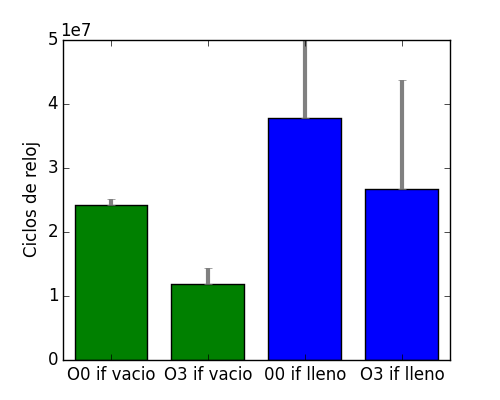
\includegraphics[scale=0.7]{images/hsl-ifs.png}
  \caption{Análisis comparativo de la cantidad de ciclos de clock que tardan los programas en procesar una imagen de $16\times 10^4$ píxeles. Se indica con una barra de error la media podada. Tamaño de la muestra: 100 imágenes.}
\end{figure}


\textit{if vacio} quiere decir que los parámetros son todos 0, y la imagen es toda negra. \textit{if lleno} quiere decir que los paremetros son 99, 0, 0 y la imagen tiene los canales (255, 150, 100).  Se puede verificar fácilmente que una tal imagen siempre entra en todos los primeros condicionales y en los últimos condicionales respectivamente.

Estos resultados realmente nos sorprendieron, ya que como se puede ver, el rendimiento cambia drásticamente aún para imágenes ``chicas''. Esto definitivamente va a cambiar como escribimos programas de aquí en adelante, ya que nos hizo darnos cuenta de cuanto afectan las comparaciones a la performance del código.
Atribuimos los resultados no solo a la mayor cantidad de comparaciones, si no tambien a la gran cantidad de saltos condicionales que intervienen en el código. Debido a esto, probablemente el branch predictor no actue de la mejor manera y no se aproveche todo el potencial del pipelining.




\subsubsection*{Experimento}
Al ver los resultados, nos propusimos cambiar la implementación de assembler. Nuestra primera versión utilizaba muchos shifts, y dado que en una clase aprendimos que el desempeño de los shifts era peor que el desempeño de los shuffles, decidimos probarlo. El resultado, como se ve en la primera imagen, no fue del todo el esperado. Sí, hubo una mejora de performance, pero no fue significativa, ni nos permitió acercarnos a la implementación en C, nuestro principal objetivo.


\begin{figure}[!hbt] 
	\centering
  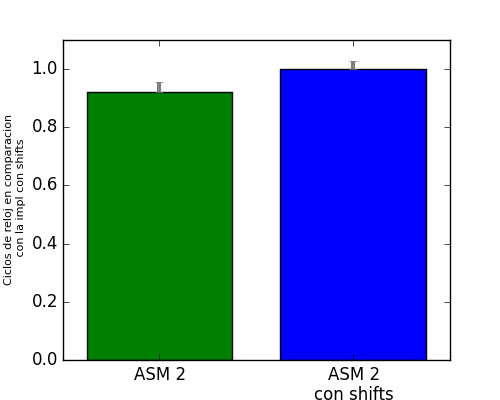
\includegraphics[scale=0.7]{images/hsl-shsh.png}
  \caption{Comparación de la cantidad de ciclos de reloj utilizada por dos variantes de hsl2. Tamaño de la muestra: 200 imágenes de $16 \times 10^4$ píxeles. Se indica el mínimo con la barra y el promedio con una linea gris.}
\end{figure}

Como se ve en esta imagen claramente, este cambio solo nos permitió un magro 10\% de ganancia sobre la implementación de C.

Algo importante que notar es que esto no significa que usar shuffles es 10\% más rápido que usar shifts, si no que es bastante más rápido. Esto se debe a que nosotros hacemos el análisis del programa completo, si se analizan por separado las partes en las que esta decisión incumbe, se llega a speedups de hasta el 40\%, dependiendo de la computadora.
\\

\subsubsection*{Experimento}
Otro experimento que se nos ocurrió realizar es la comparación entre los accesos alineados y desalinaedos a memoria. En clase aprendimos que el procesador puede optimizar los accesos alineados a memoria.
La razón de este fenómeno radica en la cache, como vimos en Organización del Computador I, a veces algunos accesos a memoria pueden ser ``a caballo'', es decir, estar en 2 lineas distintas de la cache, por lo tanto se podría llegar a 2 potenciales cache misses en un solo acceso a memoria.


Por eso es que acceder a memoria alineadamente es muy importante\footnote{http://www.ibm.com/developerworks/library/pa-dalign/} , llegando al punto que algunas arquitecturas solo permiten acceder a memoria alineadamente (de hecho la arquitectura Intel, cuando hace operaciones con registros xmm y uno de los operandos es una dirección de memoria desreferenciada, se asume que es una dirección alineada).

Sin perjucio de lo anterior, y viendo los experimentos que ya realizamos, vimos que una vez que la información está en la cache las velocidades son mucho más rápidas, y deja de importar tanto si un acceso es alineado o no, dado que la información que deseamos obtener ya esta cacheada.

Veamos los resultados:

\begin{figure}[H] 
	\centering
  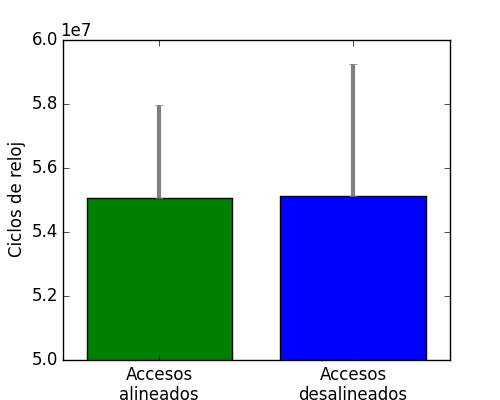
\includegraphics[scale=0.7]{images/hsl-alineamiento.png}
  \caption{Comparación de la cantidad de ciclos de reloj utilizada por dos variantes de hsl2. Tamaño de la muestra: 200 imágenes de $16 \times 10^4$ píxeles. Se indica el mínimo con la barra y el promedio con una linea gris.}
\end{figure}

Los resultados reflejan lo último que dijimos, la performance es realmente similar. Como explicamos, esto se debe a que una vez que los datos estan cacheados, no importa tanto si accedemos a ellos alineada o desalineadamente.

Sin embargo, en este experimento es interesante ponderar el caso promedio (indicado por la barra gris). Se nota que los accesos desalineados tardan más en promedio. Esto se puede deber a que, como al correr los tests la computadora esta corriendo otras tareas al mismo tiempo, debe desalojar datos de la cache y poner otros de otras tareas.

Esto provocaría que cuando nuestro programa quiera volver a obtener información que tenia previamente cacheada, deba volver a acceder a memoria principal, pagando esa penalidad. Por lo tanto, a mas grande sea la imagen y a más carga tenga el procesador (específicamente su cache), más alta va a ser la penalidad por acceder desalineadamente a memoria.

\subsubsection*{Experimento}
El último experimento que nos propusimos hacer para este código es el de comparar call vs. jmp vs. macro.

En hsl tenemos 2 subrutinas que convierten entre esquemas de colores (hslTOrgb y hslTOrgb), entonces nos encontramos con el problema de como correr ese código. En la primera variante del código (asm1), como el código de esas rutinas está escrito en C, no nos queda otra que usar calls.

Sin embargo, en la segunda versión del código, la más interesante para analizar en este experimento, nosotros tenemos que implementar las rutinas. Por lo tanto, podemos aprovecharnos de esto para ``que no nos importe'' la convención C, dado que conocemos al momento de llamar a las rutinas que registros estamos usando y que registros no, utilizar en la rutina solo aquellos que podemos pisar.

De esta manera, podríamos directamente saltar a la rutina de la tarea, ahorrandonos algunos pushs a la pila. Otra forma tambien sería pegar el código de la rutina en la rutina principal, total no pisa ningún registro importante (esta solución es exactamente la misma que la de los macros, solo que la de los macros se hace en tiempo de compilación).

Otro elemento que entra en juego es el del branch predictor: cuando hay un salto, el flujo de instrucciones posible del programa se divide en 2, y el pipeline del procesador sigue una de las ramas, que potencialmente puede ser la no tomada y entonces el procesador puede haber hecho trabajo en vano y haber perdido ciclos de reloj.

Sin embargo, como el camino que va a tomar en general es el de saltar, dado que las imagenes son grandes, va a no saltar solo una vez (la última), creemos que el efecto de este fenómeno va a ser mínimo.

\begin{figure}[H] 
	\centering
  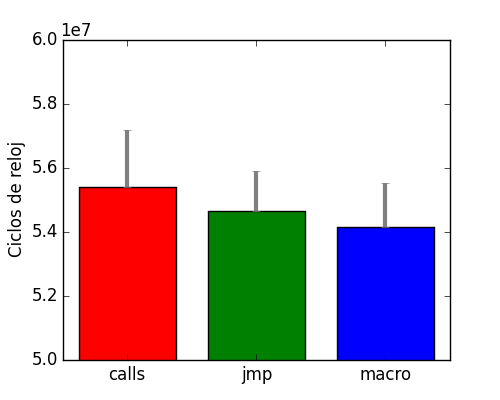
\includegraphics[scale=0.7]{images/hsl-jmpcall.png}
  \caption{Comparación de la cantidad de ciclos de reloj utilizada por dos variantes de hsl2. Tamaño de la muestra: 200 imágenes de $16 \times 10^4$ píxeles. Se indica el mínimo con la barra y el promedio con una linea gris.}
\end{figure}

Como dijimos anteriormente, para estos resultados se deben mas que nada a los overheads que tienen las operaciones de call y jmp más que a un tema de branch prediction.

El overhead del call es bastante, debe pushear la dirección de rotorno, además de algunas operaciones con la pila que hacemos al entrar a la función. Otra operatoria, no muy costosa, que tienen el call y el jmp, es la cuenta que tienen que hacer para obtener la dirección a la que tienen que saltar (nuevo IP).

Sin embargo, en terminos relativos la performance es casi igual (como se ve perfectamente en el gráfico), la diferencia entre usar calls y usar macros es de menos del 10\%.


